\chapter{Resultados}

La descomposición armónica bajo el uso de la herramienta PyTides, permite determinar los armónicos que más aportan a la componente astronómica de la marea, reconociendo su importancia en función su la amplitud. A continuación, se presentan las siete más importantes y sus respectivas amplitudes

\begin{table}[H]
\centering
\begin{tabular}{|c|c|}
	\hline
	Componente & Amplitud \\
	\hline
	M2      &  1.496 \\
	S2      &  0.421 \\
	N2      &  0.314 \\
	K1      &  0.115 \\
	K2      &  0.104 \\
	Sa      &  0.074 \\
	M4      &  0.065 \\
	\hline
\end{tabular}
\caption{Principales 7 componentes de la marea astronómica}
\label{table:componentes}
\end{table}

Según la tabla \ref{table:componentes}, las principales componentes son: principal lunar ($M_{2}$), principal solar ($S_{2}$), principal elíptica ($N_{2}$), principal menor ($K_{2})$ y principal medio-mayor ($K_{1}$); estas componentes y sus repectivos valores de amplitud son congruentes con los reportados en estudios anteriores \cite{Malikov2010}. Para clasificar el tipo de marea se calcula el coeficiente de Coutier (F) definido como:

\begin{equation}
F=\frac{ K_{1}-O_{1}}{M_{2}-S_{2}}
\end{equation}

Dónde los símbolos de cada componente representan su respectiva amplitud 

El coeficiente de Coutier, F, tiene un valor de 0.081, lo cual clasifica la marea como tipo \textbf{semidiurna} \cite{MolaresBabra2004}. Al obtener los armónicos y por tanto, la marea astronómica; se puede determinar la marea residual o meterológica.

\textcolor{red}{IMAGEN CON LOS 3 TIPOS DE MAREA DONDE SE VEA BIEN LA ONDA}

De la figura anterior, puede notarse una carrera de marea (diferencia de nivel entre la pleamar y la bajamar) cercana a los 4 metros, un valor característico en esta zona del Paćifico Colombiano. La serie residual de la marea (serie de tal color), llamada de ahora en adelante como serie de nivel del mar debido a fenómenos meteorológicos, tiene sobrelevaciones máximas diarias y la forma de determinarlas se determina a continuación:

GRAFICAS CON SOBRELEVACION




\begin{figure}[H]
	\centering
	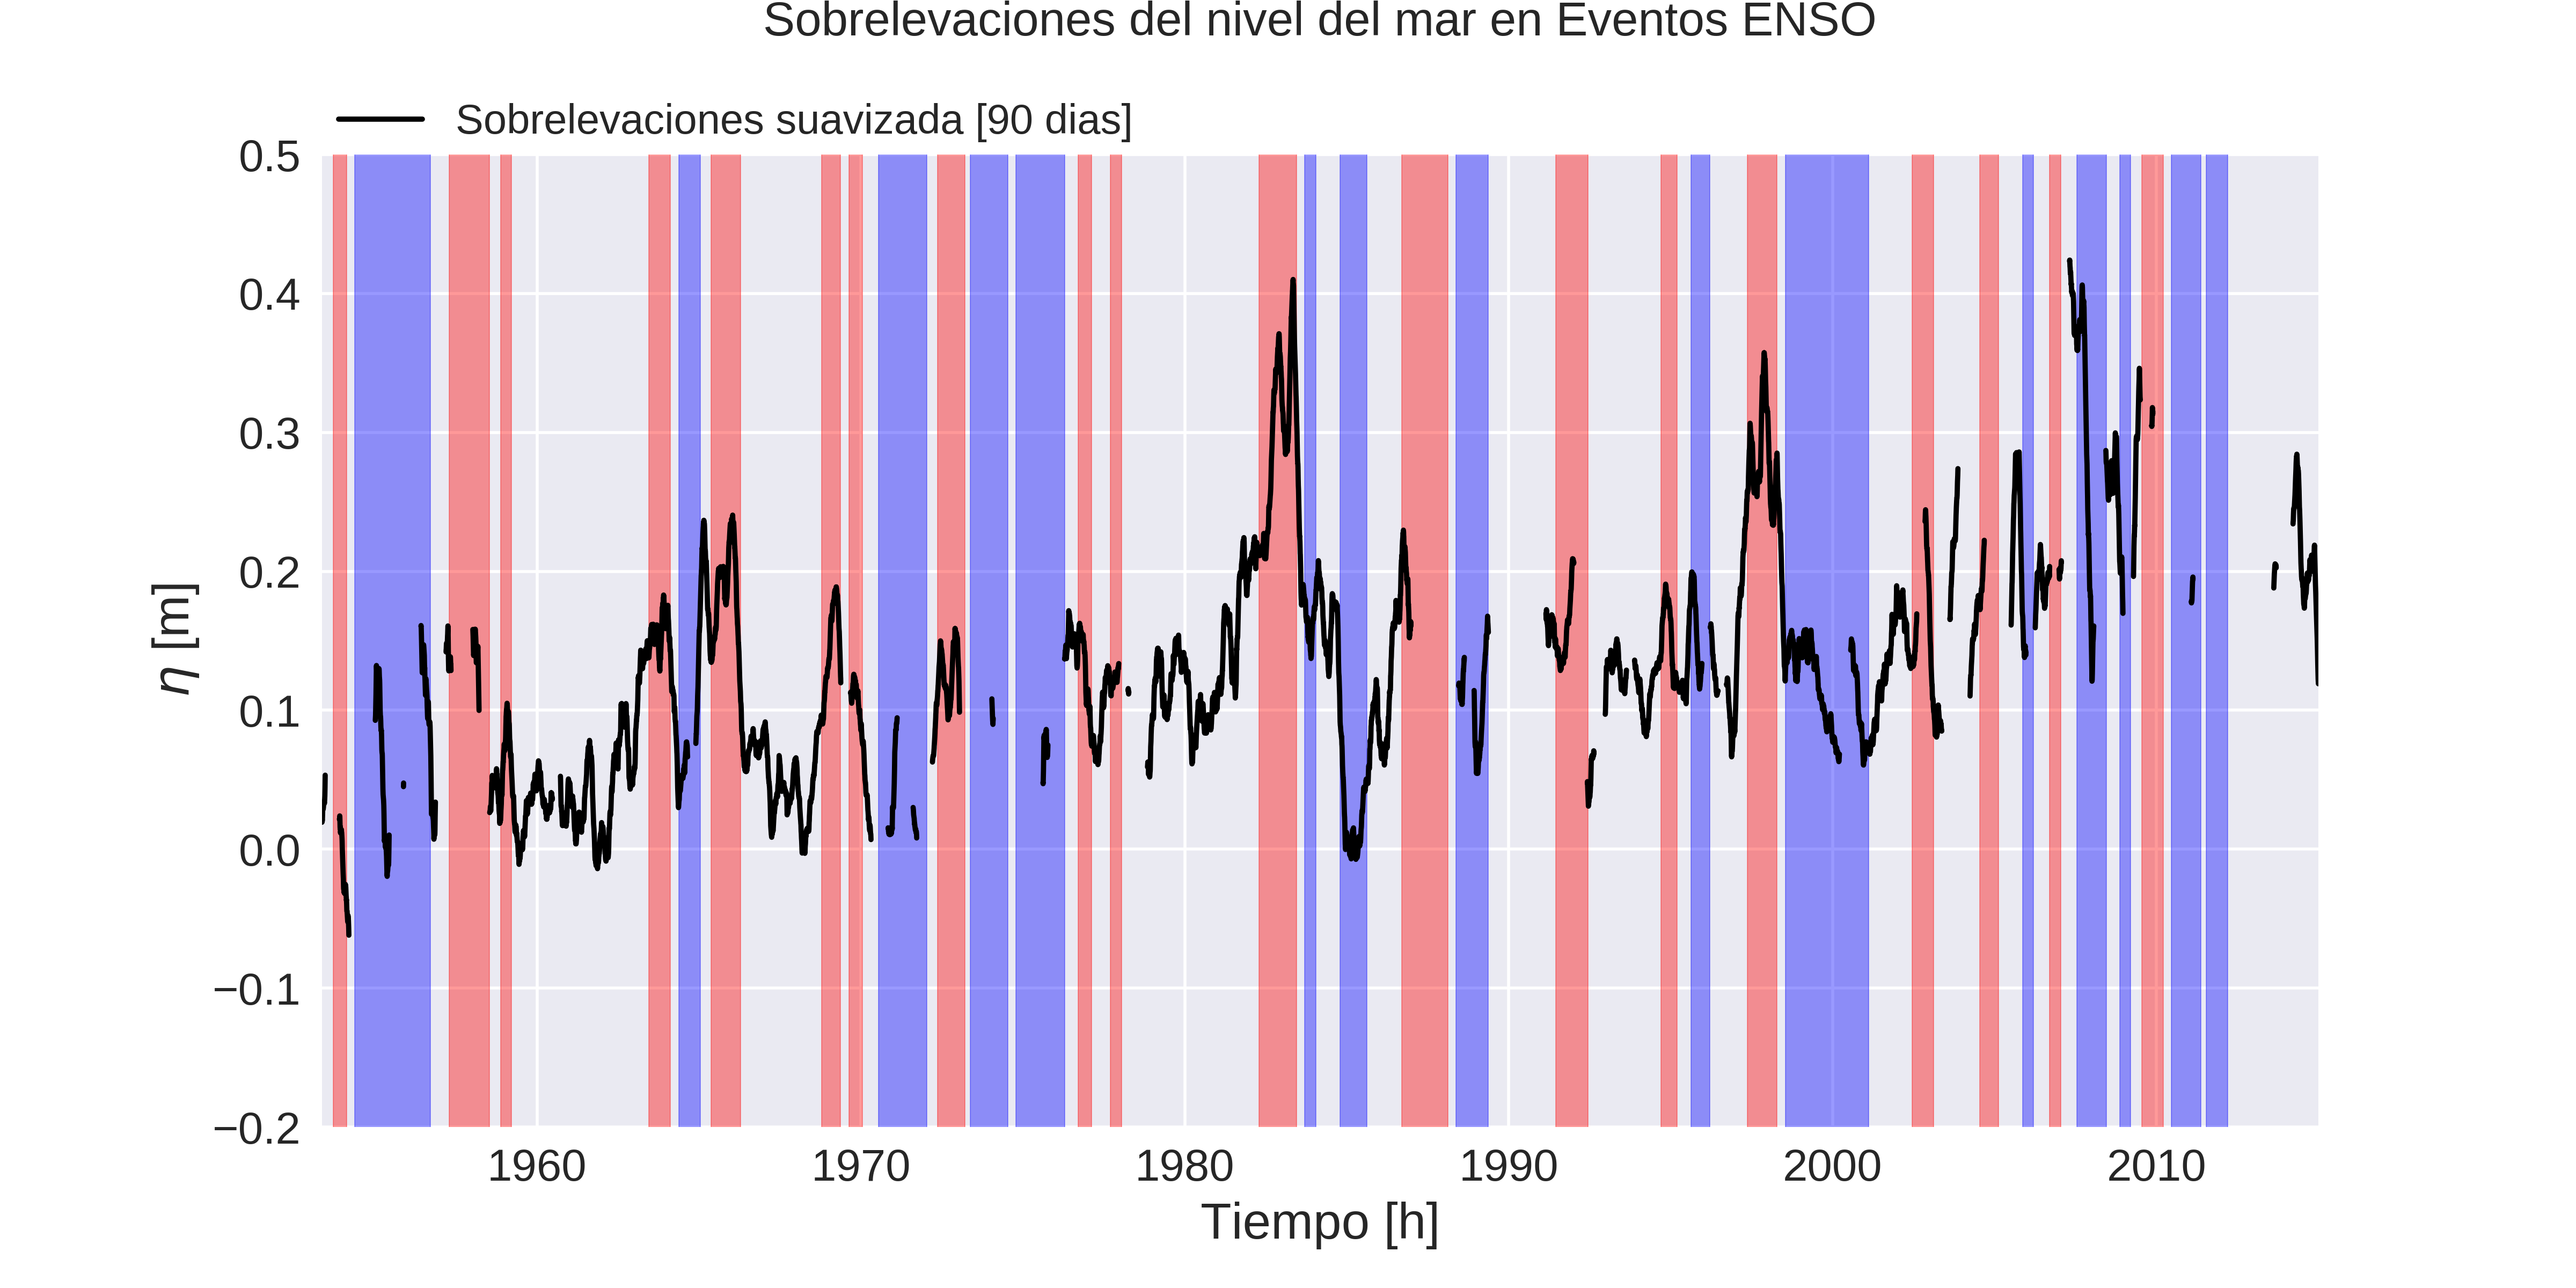
\includegraphics[width=\textwidth]{sobreelev_ENSOS.png}
	\caption{Sobrelevaciones del nivel del mar en la bahía de Buenaventura en diferentes eventos ENSOS. Las franjas rojas y azules representan fases cálidas y frías del ENSO (Eventos de Niño y Niña) }
	\label{fig:sobrelev_ENSOS}
\end{figure}






















Existen varias normas para la citaci\'{o}n bibliogr\'{a}fica. Algunas \'{a}reas del conocimiento prefieren normas espec\'{\i}ficas para citar las referencias bibliogr\'{a}ficas en el texto y escribir la lista de bibliograf\'{\i}a al final de los documentos. Esta plantilla brinda la libertad para que el autor de la tesis  o trabajo de investigaci\'{o}n utilice la norma bibliogr\'{a}fica com\'{u}n para su disciplina. Sin embargo, se solicita que la norma seleccionada se utilice con rigurosidad, sin olvidar referenciar "todos" los elementos tomados de otras fuentes (referencias bibliogr\'{a}ficas, patentes consultadas, software empleado en el manuscrito, en el tratamiento a los datos y resultados del trabajo, consultas a personas (expertos o p\'{u}blico general), entre otros).\\

\section{Ejemplos de citaciones bibliogr\'{a}ficas}
Existen algunos ejemplos para la citaci\'{o}n bibliogr\'{a}fica, por ejemplo, Microsoft Word (versiones posteriores al 2006), en el  men\'{u} de referencias, se cuenta con la opci\'{o}n de insertar citas bibliogr\'{a}ficas utilizando la norma APA (American Psychological Association) u otras normas y con la ayuda para construir autom\'{a}ticamente la lista al final del documento. De la misma manera, existen administradores bibliogr\'{a}ficos compatibles con Microsoft Word como Zotero, End Note y el Reference Manager,  disponibles a trav\'{e}s del Sistema Nacional de Bibliotecas (SINAB) de la Universidad Nacional de Colombia\footnote{Ver:www.sinab.unal.edu.co } secci\'{o}n "Recursos bibliogr\'{a}ficos" opci\'{o}n "Herramientas Bibliogr\'{a}ficas. A continuaci\'{o}n se muestra un ejemplo de una de las formas m\'{a}s usadas para las citaciones bibliogr\'{a}ficas.\\

Citaci\'{o}n individual:\cite{AG01}.\\
Citaci\'{o}n simult\'{a}nea de varios autores:
\cite{AG12,AG52,AG70,AG08a,AG09a,AG36a,AG01i}.\\

Por lo general, las referencias bibliogr\'{a}ficas correspondientes a los anteriores n\'{u}meros, se listan al final del documento en orden de aparici\'{o}n o en orden alfab\'{e}tico. Otras normas de citaci\'{o}n incluyen el apellido del autor y el a\~{n}o de la referencia, por ejemplo: 1) "...\'{e}nfasis en elementos ligados al \'{a}mbito ingenieril que se enfocan en el manejo de datos e informaci\'{o}n estructurada y que seg\'{u}n Kostoff (1997) ha atra\'{\i}do la atenci\'{o}n de investigadores dado el advenimiento de TIC...", 2) "...Dicha afirmaci\'{o}n coincide con los planteamientos de Snarch (1998), citado por Castellanos (2007), quien comenta que el manejo..." y 3) "...el futuro del sistema para argumentar los procesos de toma de decisiones y el desarrollo de ideas innovadoras (Nosella \textsl{et al}., 2008)...".\\

\section{Ejemplos de presentaci\'{o}n y citaci\'{o}n de figuras}
Las ilustraciones forman parte del contenido de los cap\'{\i}tulos. Se deben colocar en la misma p\'{a}gina en que se mencionan o en la siguiente (deben siempre mencionarse en el texto).\\

Las llamadas para explicar alg\'{u}n aspecto de la informaci\'{o}n deben hacerse con nota al pie y su nota correspondiente\footnote{Las notas van como "notas al pie". Se utilizan para explicar, comentar o hacer referencia al texto de un documento, as\'{\i} como para introducir comentarios detallados y en ocasiones para citar fuentes de informaci\'{o}n (aunque para esta opci\'{o}n es mejor seguir en detalle las normas de citaci\'{o}n bibliogr\'{a}fica seleccionadas).}. La fuente documental se debe escribir al final de la ilustraci\'{o}n o figura con los elementos de la referencia (de acuerdo con las normas seleccionadas) y no como pie de p\'{a}gina. Un ejemplo para la presentaci\'{o}n y citaci\'{o}n de figuras, se presenta a continuaci\'{o}n (citaci\'{o}n directa):\\

Por medio de las propiedades del fruto, seg\'{u}n el espesor del endocarpio, se hace una clasificaci\'{o}n de la palma de aceite en tres tipos: Dura, Ternera y Pisifera, que se ilustran en la Figura
\ref{fig:Fruto}.\\
\begin{figure}
\centering%
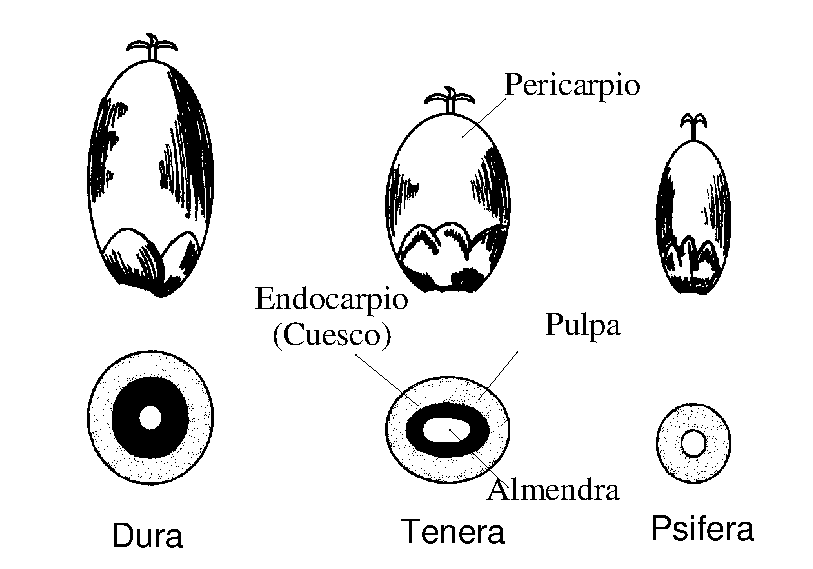
\includegraphics{Kap3/FrutoSp}%
\caption{Tipos y partes del fruto de palma de aceite \cite{AG03p,AG04p}.} \label{fig:Fruto}
\end{figure}

\section{Ejemplo de presentaci\'{o}n y citaci\'{o}n de tablas y cuadros}
Para la edici\'{o}n de tablas, cada columna debe llevar su t\'{\i}tulo; la primera palabra se debe escribir con may\'{u}scula inicial y preferiblemente sin abreviaturas. En las tablas y cuadros, los t\'{\i}tulos y datos se deben ubicar entre l\'{\i}neas horizontales y verticales cerradas (como se realiza en esta plantilla).\\

La numeraci\'{o}n de las tablas se realiza de la misma manera que las figuras o ilustraciones, a lo largo de todo el texto. Deben llevar un t\'{\i}tulo breve, que concreta el contenido de la tabla; \'{e}ste se debe escribir en la parte superior de la misma. Para la presentaci\'{o}n de cuadros, se deben seguir las indicaciones dadas para las tablas.\\

Un ejemplo para la presentaci\'{o}n y citaci\'{o}n de tablas (citaci\'{o}n indirecta), se presenta a continuaci\'{o}n:\\

De esta participaci\'{o}n aproximadamente el 60 \% proviene de biomasa
(Tabla \ref{EMundo1}).
\begin{center}
\begin{threeparttable}
\centering%
\caption{Participaci\'{o}n de las energ\'{\i}as renovables en el suministro
total de energ\'{\i}a primaria \cite{AG02i}.}\label{EMundo1}
\begin{tabular}{|l|c|c|}\hline
&\multicolumn{2}{c|}{Participaci\'{o}n en el suministro de energ\'{\i}a primaria /\% (Mtoe)\;$\tnote{1}$}\\\cline{2-3}%
\arr{Region}&Energ\'{\i}as renovables &Participaci\'{o}n de la biomasa\\\hline%
Latinoam\'{e}rica&28,9 (140)&62,4 (87,4)\\\hline%
\:Colombia&27,7 (7,6)&54,4 (4,1)\\\hline%
Alemania&3,8 (13,2)&65,8 (8,7)\\\hline%
Mundial&13,1 (1404,0)&79,4 (1114,8)\\\hline
\end{tabular}
\begin{tablenotes}
\item[1] \footnotesize{1 kg oe=10000 kcal=41,868 MJ}
\end{tablenotes}
\end{threeparttable}
\end{center}

NOTA: en el caso en que el contenido de la tabla o cuadro sea muy extenso, se puede cambiar el tama\~{n}o de la letra, siempre y cuando \'{e}sta sea visible por el lector.\\

\subsection{Consideraciones adicionales para el manejo de figuras y tablas}
Cuando una tabla, cuadro o figura ocupa m\'{a}s de una p\'{a}gina, se debe repetir su identificaci\'{o}n num\'{e}rica, seguida por la palabra continuaci\'{o}n.\\

Adicionalmente los encabezados de las columnas se deben repetir en todas las p\'{a}ginas despu\'{e}s de la primera.\\

Los anteriores lineamientos se contemplan en la presente plantilla.\\

\begin{itemize}
\item Presentaci\'{o}n y citaci\'{o}n de ecuaciones.
\end{itemize}

La citaci\'{o}n de ecuaciones, en caso que se presenten, debe hacerse como lo sugiere esta plantilla. Todas las ecuaciones deben estar numeradas y citadas detro del texto.\\

Para el manejo de cifras se debe seleccionar la norma seg\'{u}n el \'{a}rea de conocimiento de la tesis  o trabajo de investigaci\'{o}n.\\